\chapter{Architectures: Graph Neural Networks}
\label{sec:arch-gnn}

A graph neural network (GNN) updates an entity by combining its current representation with information from entities connected to it.
The architecture therefore makes a structural choice before learning begins: \emph{which pairs of entities are allowed to exchange information?}
For a CNN that relation is a fixed local image grid; for a Transformer it is commonly a dense or masked attention pattern; for a GNN it is supplied or constructed as a graph.

\begin{figure}[htbp]
\centering
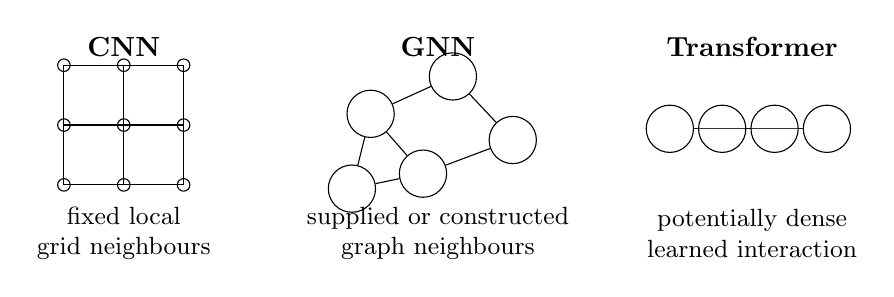
\begin{tikzpicture}[scale=0.95, every node/.style={font=\small}]
  % CNN
  \node[font=\bfseries] at (-4.2,2.05) {CNN};
  \foreach \x in {-5.0,-4.2,-3.4} {
    \foreach \y in {0.2,1.0,1.8} {
      \node[circle,draw,inner sep=1.6pt] (c\x\y) at (\x,\y) {};
    }
  }
  \foreach \x in {-5.0,-4.2,-3.4} {
    \draw (\x,0.2)--(\x,1.0)--(\x,1.8);
  }
  \foreach \y in {0.2,1.0,1.8} {
    \draw (-5.0,\y)--(-4.2,\y)--(-3.4,\y);
  }
  \node[align=center] at (-4.2,-0.45) {fixed local\\grid neighbours};

  % GNN
  \node[font=\bfseries] at (0,2.05) {GNN};
  \node[circle,draw,minimum size=6mm] (g1) at (-0.9,1.15) {};
  \node[circle,draw,minimum size=6mm] (g2) at (0.2,1.65) {};
  \node[circle,draw,minimum size=6mm] (g3) at (1.0,0.8) {};
  \node[circle,draw,minimum size=6mm] (g4) at (-0.2,0.35) {};
  \node[circle,draw,minimum size=6mm] (g5) at (-1.15,0.15) {};
  \draw (g1)--(g2)--(g3)--(g4)--(g1);
  \draw (g4)--(g5)--(g1);
  \node[align=center] at (0,-0.45) {supplied or constructed\\graph neighbours};

  % Transformer
  \node[font=\bfseries] at (4.2,2.05) {Transformer};
  \foreach \i/\x in {1/3.1,2/3.8,3/4.5,4/5.2} {
    \node[circle,draw,minimum size=6mm] (t\i) at (\x,0.95) {};
  }
  \foreach \i in {1,...,4} {
    \foreach \j in {1,...,4} {
      \ifnum\i<\j\relax\draw[opacity=0.55] (t\i)--(t\j);\fi
    }
  }
  \node[align=center] at (4.2,-0.45) {potentially dense\\learned interaction};
\end{tikzpicture}
\caption{Three interaction biases. CNNs hard-code a regular local neighbourhood, GNNs communicate along graph edges, and dense self-attention can make every element a candidate interaction. The difference is primarily an information-routing choice.}
\label{fig:gnn-cnn-transformer}
\end{figure}

\begin{calloutintuition}
A GNN is a neural network whose communication routes are a graph.
\end{calloutintuition}

\section{Graph representation: entities, relations and features}
A graph contains a set of nodes $\mathcal V$ and edges $\mathcal E$.
For learning, nodes usually carry features $x_i$, edges may carry features $e_{ij}$, and the complete graph may carry global context $u$.
The adjacency structure says which node pairs are connected; unlike an image grid, the number and arrangement of neighbours can vary from node to node.

\[
\underbrace{G}_{\text{one graph}}
=
\left(
\underbrace{\{x_i\}_{i\in\mathcal V}}_{\text{node information}},
\underbrace{\{(i,j,e_{ij})\}_{(i,j)\in\mathcal E}}_{\text{relations / edge information}},
\underbrace{u}_{\text{optional graph context}}
\right).
\]

An edge may mean a chemical bond, road connection, social interaction, mesh adjacency, physical contact or a relation in a knowledge graph.
That meaning matters because the graph itself is part of the model's prior structure rather than merely a storage format.
Directed graphs distinguish $i\rightarrow j$ from $j\rightarrow i$; heterogeneous graphs may additionally distinguish node and edge types, so a relation such as \texttt{author-of} need not share parameters with \texttt{cites}.

\begin{figure}[htbp]
\centering
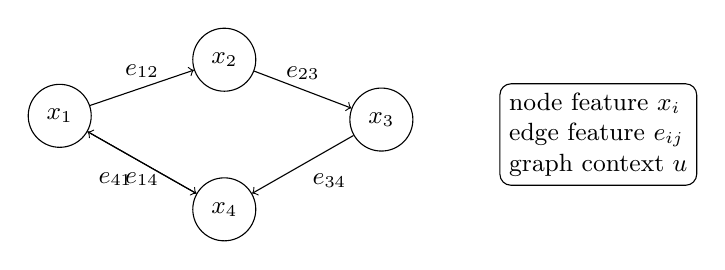
\begin{tikzpicture}[scale=0.95, every node/.style={font=\small}]
  \node[circle,draw,minimum size=8mm] (a) at (-2.2,0.6) {$x_1$};
  \node[circle,draw,minimum size=8mm] (b) at (0,1.35) {$x_2$};
  \node[circle,draw,minimum size=8mm] (c) at (2.1,0.55) {$x_3$};
  \node[circle,draw,minimum size=8mm] (d) at (0,-0.65) {$x_4$};
  \draw[->] (a)--node[above] {$e_{12}$}(b);
  \draw[->] (b)--node[above] {$e_{23}$}(c);
  \draw[->] (c)--node[below right] {$e_{34}$}(d);
  \draw[->] (d)--node[below left] {$e_{41}$}(a);
  \draw[->] (a)--node[below] {$e_{14}$}(d);
  \node[draw,rounded corners,align=left] at (5.0,0.35) {
    node feature $x_i$\\
    edge feature $e_{ij}$\\
    graph context $u$
  };
\end{tikzpicture}
\caption{The graph gives both values and routing structure. Node features describe entities; edge features can describe the relation through which information travels.}
\label{fig:gnn-graph-representation}
\end{figure}

\subsection{Graph construction.}
Sometimes the graph is observed directly, such as bonds in a molecule or links in a road network.
Sometimes it is a modelling choice: connect spatial points within a radius, connect each point to its $N_{\text{neighbours}}$ nearest neighbours, or learn an affinity from representations.
This distinction is important because changing the graph changes which information can meet before any neural parameter changes.

\section{Message passing: the core operation}
Most classical GNNs can be understood as repeated \textbf{message passing}.
For node $i$, each neighbour $j$ creates a message, the incoming messages are aggregated, and the result updates the node representation:

\[
\begin{aligned}
\underbrace{m_i^{(\ell)}}_{\text{incoming neighbourhood information}}
&=
\operatorname{Aggregate}_{j\in\mathcal N(i)}
\left[
\operatorname{Message}_{\theta}
\left(
\underbrace{h_i^{(\ell)}}_{\text{receiver}},
\underbrace{h_j^{(\ell)}}_{\text{sender}},
\underbrace{e_{ij}}_{\text{relation}}
\right)
\right],\\[1mm]
\underbrace{h_i^{(\ell+1)}}_{\text{new node representation}}
&=
\operatorname{Update}_{\theta}
\left(
\underbrace{h_i^{(\ell)}}_{\text{current node state}},
\underbrace{m_i^{(\ell)}}_{\text{neighbour summary}}
\right).
\end{aligned}
\]

The graph chooses the candidate senders $\mathcal N(i)$; the neural functions decide what information those senders contribute and how the receiver changes.
A self-loop or explicit residual path lets the node preserve its own information instead of replacing it with a pure neighbourhood summary.

\begin{figure}[htbp]
\centering
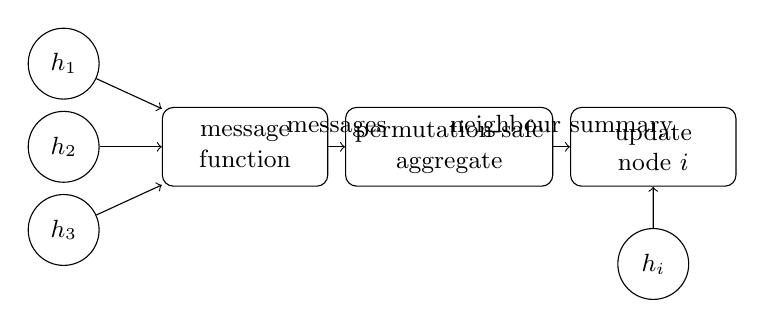
\begin{tikzpicture}[scale=0.96, every node/.style={font=\small}]
  \node[circle,draw,minimum size=9mm] (n1) at (-4,1.1) {$h_1$};
  \node[circle,draw,minimum size=9mm] (n2) at (-4,0) {$h_2$};
  \node[circle,draw,minimum size=9mm] (n3) at (-4,-1.1) {$h_3$};
  \node[draw,rounded corners,minimum width=2.1cm,minimum height=1.0cm,align=center] (msg) at (-1.6,0) {message\\function};
  \node[draw,rounded corners,minimum width=2.1cm,minimum height=1.0cm,align=center] (agg) at (1.1,0) {permutation-safe\\aggregate};
  \node[draw,rounded corners,minimum width=2.1cm,minimum height=1.0cm,align=center] (upd) at (3.8,0) {update\\node $i$};
  \draw[->] (n1)--(msg);
  \draw[->] (n2)--(msg);
  \draw[->] (n3)--(msg);
  \draw[->] (msg)--node[above] {messages}(agg);
  \draw[->] (agg)--node[above] {neighbour summary}(upd);
  \node[circle,draw,minimum size=9mm] (self) at (3.8,-1.55) {$h_i$};
  \draw[->] (self)--(upd);
\end{tikzpicture}
\caption{One message-passing layer. Neighbour states are transformed into messages, combined without depending on arbitrary neighbour order, then merged with the receiver state.}
\label{fig:gnn-message-passing}
\end{figure}

\subsection{The main research split.}
Papers that appear to propose very different GNNs often modify only one of four places: the graph, the message, the aggregation rule, or the update/readout.
This decomposition is more useful than memorising model names because it identifies the actual design change.

\section{Depth is graph distance}
One message-passing layer lets a node use one-hop neighbours.
Two layers allow information from nodes two edges away to arrive through an intermediate node; after $L$ layers, a node can usually depend on its $L$-hop neighbourhood.
Depth therefore controls both neural transformation and communication distance.

\begin{figure}[htbp]
\centering
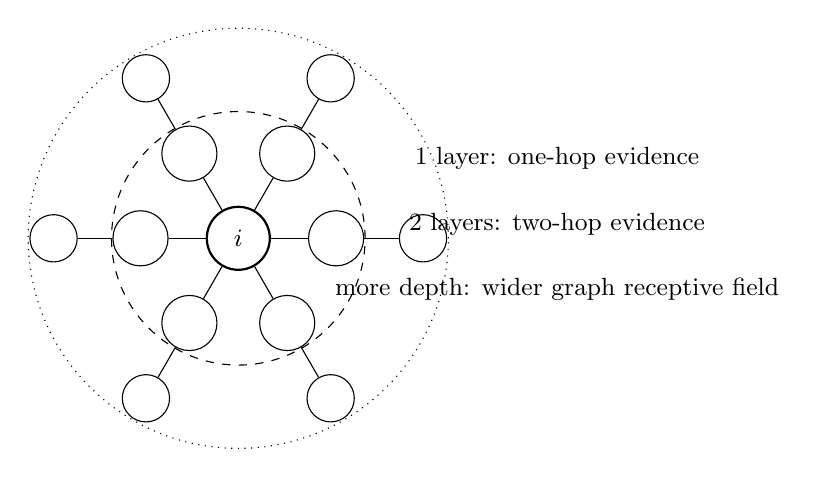
\begin{tikzpicture}[scale=0.92, every node/.style={font=\small}]
  \node[circle,draw,thick,minimum size=8mm] (c) at (0,0) {$i$};
  \foreach \a/\name in {0/a,60/b,120/c1,180/d,240/e,300/f} {
    \node[circle,draw,minimum size=7mm] (\name) at (\a:1.35) {};
    \draw (c)--(\name);
  }
  \foreach \parent/\ang/\child in {a/0/a2,b/60/b2,c1/120/c2,d/180/d2,e/240/e2,f/300/f2} {
    \node[circle,draw,minimum size=6mm] (\child) at (\ang:2.55) {};
    \draw (\parent)--(\child);
  }
  \draw[dashed] (0,0) circle (1.75);
  \draw[dotted] (0,0) circle (2.9);
  \node[align=left] at (4.4,1.1) {1 layer: one-hop evidence};
  \node[align=left] at (4.4,0.2) {2 layers: two-hop evidence};
  \node[align=left] at (4.4,-0.7) {more depth: wider graph receptive field};
\end{tikzpicture}
\caption{Graph depth expands a node's receptive field by graph distance rather than Euclidean distance or sequence position.}
\label{fig:gnn-receptive-field}
\end{figure}

This is analogous to CNN receptive fields in Section~12, but graph distance follows connectivity rather than pixels.
A long graph path can separate physically close nodes, while one edge can connect geometrically distant entities.

\begin{calloutintuition}
GNN depth is communication distance: $L$ message-passing layers expose roughly an $L$-hop neighbourhood.
\end{calloutintuition}

\section{Permutation symmetry: node numbers should not matter}
Node IDs normally have no semantic ordering.
Renumbering the same graph should therefore renumber node-level outputs consistently, while a graph-level prediction should remain unchanged.
If $P$ is a permutation matrix, a node-level GNN should satisfy the equivariance relation

\[
\underbrace{f(PX,\,PAP^\top)}_{\text{same graph with reordered node IDs}}
=
\underbrace{P f(X,A)}_{\text{same node outputs, reordered}}.
\]

For a graph-level readout $r$, the corresponding requirement is invariance:

\[
\underbrace{r(PH)}_{\text{reordered nodes}}
=
\underbrace{r(H)}_{\text{same graph prediction}}.
\]

Sum, mean and max are useful aggregation operations because their result does not depend on the order in which neighbours are presented.
Concatenating neighbours in arbitrary storage order would instead make node numbering part of the function.

\subsection{Inductive bias.}
If node identity is arbitrary but relations are meaningful, permutation equivariance lets one learned local rule operate anywhere in the graph.
If absolute node identity itself carries information, that information must be represented explicitly rather than accidentally through array position.

\section{GCN: normalised neighbour mixing}
A Graph Convolutional Network (GCN) makes message passing deliberately simple: add self-connections, mix neighbouring features with degree normalisation, then apply a learned feature transform.
A common layer is

\[
\begin{aligned}
\widetilde A&=A+I,\\
\underbrace{H^{(\ell+1)}}_{\text{updated node representations}}
&=
\phi\!\left(
\underbrace{\widetilde D^{-1/2}\widetilde A\widetilde D^{-1/2}}_{\text{normalised graph mixing}}
\underbrace{H^{(\ell)}\theta_{\text{features}}^{(\ell)}}_{\text{learned feature transform}}
\right).
\end{aligned}
\]

Degree normalisation prevents high-degree nodes from automatically producing proportionally larger summed activations merely because they have more neighbours.
The layer is therefore a learned feature transform wrapped around a graph smoothing operation.
That bias is useful when connected nodes should share information, but repeated smoothing becomes a failure mode when neighbours should remain distinct.

\begin{calloutintuition}
GCN = learn features while repeatedly smoothing them across graph edges.
\end{calloutintuition}

\section{GraphSAGE: sample and aggregate}
Full-neighbour aggregation becomes expensive when high-degree nodes connect to thousands or millions of neighbours.
GraphSAGE makes the neighbourhood itself part of the approximation: sample a bounded set of neighbours, aggregate their states, and combine the result with the target node.

\[
\begin{aligned}
\underbrace{\widehat{\mathcal N}(i)}_{\text{sampled neighbours}}
&\subseteq
\underbrace{\mathcal N(i)}_{\text{all neighbours}},\\[-1mm]
&\text{bounded work}
\quad\leftrightarrow\quad
\text{incomplete / noisier neighbourhood evidence}.
\end{aligned}
\]

GraphSAGE is also associated with \textbf{inductive} use: the model learns an aggregation rule from features rather than storing only one learned embedding per training node, so it can process previously unseen nodes when their features and neighbourhood are available.
This does not mean every GraphSAGE setup generalises automatically; the new graph must still resemble the training regime in the ways the learned rule relies on.

\begin{figure}[htbp]
\centering
\begin{tikzpicture}[scale=0.9, every node/.style={font=\small}]
  \node[font=\bfseries] at (-3.3,2.0) {Full neighbourhood};
  \node[circle,draw,thick,minimum size=8mm] (f0) at (-3.3,0.7) {$i$};
  \foreach \a/\k in {0/1,45/2,90/3,135/4,180/5,225/6,270/7,315/8} {
    \node[circle,draw,minimum size=5mm] (f\k) at ($(-3.3,0.7)+(\a:1.1)$) {};
    \draw (f0)--(f\k);
  }
  \node[font=\bfseries] at (3.1,2.0) {Sampled neighbourhood};
  \node[circle,draw,thick,minimum size=8mm] (s0) at (3.1,0.7) {$i$};
  \foreach \a/\k in {20/1,105/2,210/3,300/4} {
    \node[circle,draw,minimum size=5mm] (s\k) at ($(3.1,0.7)+(\a:1.1)$) {};
    \draw[thick] (s0)--(s\k);
  }
  \node at (0,-1.0) {$\text{less work} \;\leftrightarrow\; \text{less complete local evidence}$};
\end{tikzpicture}
\caption{Neighbour sampling bounds compute and memory, but the sampled subgraph is an estimator of the full neighbourhood rather than the full neighbourhood itself.}
\label{fig:gnn-neighbour-sampling}
\end{figure}

\section{GAT: learn which neighbours matter}
A Graph Attention Network (GAT) keeps graph edges as the set of allowed interactions but learns how strongly each permitted neighbour contributes.
For node $i$,

\[
\begin{aligned}
\underbrace{\alpha_{ij}}_{\text{importance of neighbour }j}
&=
\operatorname{softmax}_{j\in\mathcal N(i)}
\left(
\underbrace{\operatorname{score}_{\theta}(h_i,h_j,e_{ij})}_{\text{content / relation compatibility}}
\right),\\[1mm]
\underbrace{h_i'}_{\text{updated node}}
&=
\phi\!\left(
\sum_{j\in\mathcal N(i)}
\alpha_{ij}\,\theta_{\text{value}}h_j
\right).
\end{aligned}
\]

This is conceptually close to attention in Section~13.1, but the graph commonly supplies a sparse mask: only connected nodes compete for attention weight.
The graph therefore says \emph{who may speak}; attention decides \emph{who matters for this update}.
Multi-head graph attention adds the same broad optionality as multi-head Transformer attention: different heads can represent different relation patterns, at additional memory and compute cost.

\begin{figure}[htbp]
\centering
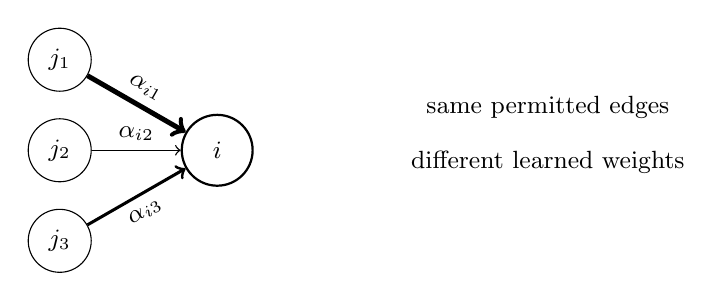
\begin{tikzpicture}[scale=1.0, every node/.style={font=\small}]
  \node[circle,draw,thick,minimum size=9mm] (i) at (0,0) {$i$};
  \node[circle,draw,minimum size=8mm] (a) at (-2,1.15) {$j_1$};
  \node[circle,draw,minimum size=8mm] (b) at (-2,0) {$j_2$};
  \node[circle,draw,minimum size=8mm] (c) at (-2,-1.15) {$j_3$};
  \draw[->,line width=1.8pt] (a)--node[above,sloped] {$\alpha_{i1}$}(i);
  \draw[->,line width=0.5pt] (b)--node[above,sloped] {$\alpha_{i2}$}(i);
  \draw[->,line width=1.1pt] (c)--node[below,sloped] {$\alpha_{i3}$}(i);
  \node[align=left] at (4.2,0.55) {same permitted edges};
  \node[align=left] at (4.2,-0.15) {different learned weights};
\end{tikzpicture}
\caption{Graph attention learns importance inside the allowed neighbourhood. Edge thickness represents a larger or smaller learned contribution, not a change in connectivity.}
\label{fig:gnn-gat}
\end{figure}

\section{GCN, GraphSAGE and GAT are choices inside one mechanism}
The model names are less important than the message-passing choices they instantiate.

\begin{table}[htbp]
\centering
\small
\begin{tabular}{p{0.14\textwidth}p{0.21\textwidth}p{0.23\textwidth}p{0.26\textwidth}}
\toprule
Method & Neighbour rule & What it buys & Main cost / assumption \\
\midrule
GCN & normalised mixing over graph neighbours & simple, efficient local smoothing & connected nodes should benefit from mixing; full neighbourhood may be costly \\
GraphSAGE & sample neighbours, then aggregate & bounded neighbourhood work; natural inductive use & sampling variance and missed neighbours \\
GAT & learned attention over allowed neighbours & content-dependent neighbour importance & extra scoring work; edges still constrain candidate interactions \\
General MPNN & learned message + aggregation + update & flexible node/edge interaction design & more capacity and more ways to overfit or spend compute \\
\bottomrule
\end{tabular}
\caption{Several common GNN families differ mainly in how they construct and weight messages, not in the broad data flow.}
\label{tab:gnn-families}
\end{table}

\section{MPNN: the general abstraction}
A Message Passing Neural Network (MPNN) treats the message function itself as learnable and may use edge features explicitly.
For molecular graphs, for example, the message from atom $j$ to atom $i$ can depend on the sender representation, receiver representation and bond type rather than only a scalar adjacency entry.
The same abstraction covers many architectures:

\[
\boxed{
\text{graph construction}
\rightarrow
\text{message}
\rightarrow
\text{aggregate}
\rightarrow
\text{update}
\rightarrow
\text{readout}
}
\]

When reading a GNN paper, first locate which arrow changed.
A new name can hide a small local architectural change; conversely, a change to graph construction or symmetry constraints can alter the hypothesis class substantially even if the neural block looks familiar.

\section{Expressivity: aggregation can destroy distinctions}
Permutation-safe aggregation deliberately compresses a set of neighbour states into one vector.
Compression creates collisions: two different neighbourhoods can produce the same aggregate, after which later layers cannot reconstruct which neighbourhood was present.
For example, a simple mean discards neighbour count when two multisets have the same average.

Many standard message-passing GNNs are closely related in distinguishing power to the one-dimensional Weisfeiler--Lehman (1-WL) graph-refinement procedure: some non-isomorphic graph structures remain indistinguishable regardless of training.
The practical consequence is not that message passing is weak in general; it is that architecture-level symmetry and aggregation choices bound what structure can ever become visible to the predictor.
Higher-order, subgraph, positional-encoding and graph-Transformer methods add information specifically to break some of these collisions, usually at increased compute or reduced symmetry simplicity.

\begin{calloutintuition}
Aggregation buys permutation symmetry by throwing information away; expressivity depends on what survives that compression.
\end{calloutintuition}

\section{Prediction level: node, edge or whole graph}
The same message-passing backbone can support different prediction targets.
A node task reads one or more node states; an edge task scores a pair of node states; a graph task first compresses all node states into one graph representation.

\begin{figure}[htbp]
\centering
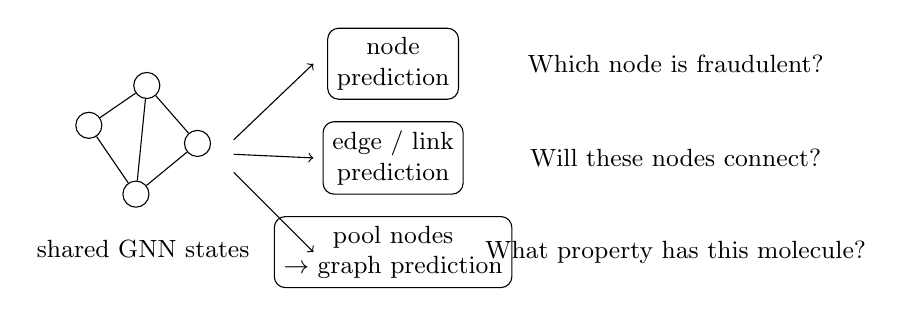
\begin{tikzpicture}[scale=0.92, every node/.style={font=\small}]
  \node[circle,draw] (a) at (-4,0.7) {};
  \node[circle,draw] (b) at (-3.2,1.25) {};
  \node[circle,draw] (c) at (-2.5,0.45) {};
  \node[circle,draw] (d) at (-3.35,-0.25) {};
  \draw (a)--(b)--(c)--(d)--(a);
  \draw (b)--(d);
  \node at (-3.25,-1.0) {shared GNN states};

  \draw[->] (-2.0,0.5)--(-0.9,1.55);
  \node[draw,rounded corners,align=center] at (0.2,1.55) {node\\prediction};

  \draw[->] (-2.0,0.3)--(-0.9,0.25);
  \node[draw,rounded corners,align=center] at (0.2,0.25) {edge / link\\prediction};

  \draw[->] (-2.0,0.05)--(-0.9,-1.05);
  \node[draw,rounded corners,align=center] at (0.2,-1.05) {pool nodes\\$\rightarrow$ graph prediction};

  \node[align=left] at (4.1,1.55) {Which node is fraudulent?};
  \node[align=left] at (4.1,0.25) {Will these nodes connect?};
  \node[align=left] at (4.1,-1.05) {What property has this molecule?};
\end{tikzpicture}
\caption{Prediction level changes the readout, not necessarily the message-passing backbone.}
\label{fig:gnn-prediction-levels}
\end{figure}

\subsection{Link prediction.}
A link score often uses a dot product, bilinear score or small neural function of two node states.
Negative examples are usually far more numerous than observed positive edges, so the negative-sampling policy becomes part of the training problem rather than a harmless implementation detail.

\section{Pooling: many nodes to one graph state}
Graph-level prediction needs a permutation-invariant readout.
Common choices expose different information:

\begin{table}[htbp]
\centering
\small
\begin{tabular}{p{0.18\textwidth}p{0.32\textwidth}p{0.38\textwidth}}
\toprule
Readout & Preserves / emphasises & Main consequence \\
\midrule
Sum & accumulated evidence and graph size & can represent counts; magnitude grows with node count \\
Mean & average node evidence & normalises graph size but can erase count information \\
Max & strongest feature presence & detects whether a strong local signal exists; ignores multiplicity \\
Learned pooling & task-dependent selection / coarsening & more expressive compression but adds parameters and possible instability \\
\bottomrule
\end{tabular}
\caption{Pooling is an information-compression choice. No readout is universally best because each preserves different graph statistics.}
\label{tab:gnn-pooling}
\end{table}

Hierarchical pooling instead produces progressively coarser graphs, analogous to reducing spatial resolution in a CNN.
The useful question is what information may safely disappear when many local states become one global state.

\section{The central inductive bias}
A GNN assumes that the supplied relation structure identifies useful routes for sharing information and that some update rule can be reused across many nodes or edges.
This can give strong data efficiency when the graph matches the mechanism generating the target.
It can also hard-code the wrong interactions when the supplied topology is noisy, missing, adversarial or simply unrelated to the prediction target.

\begin{table}[htbp]
\centering
\small
\begin{tabular}{p{0.16\textwidth}p{0.34\textwidth}p{0.38\textwidth}}
\toprule
Architecture & Structural preference / assumption & Useful regime \\
\midrule
CNN & nearby grid positions contain reusable local patterns & images and other regular spatial grids \\
GNN & connected entities should exchange information through reusable relation-aware rules & molecules, networks, meshes, relational data \\
Transformer & useful interactions can be selected largely from content, often among many candidate pairs & sequences / sets with flexible long-range interaction \\
\bottomrule
\end{tabular}
\caption{CNNs, GNNs and Transformers differ mainly in how strongly the architecture constrains the interaction graph before learning.}
\label{tab:gnn-inductive-bias}
\end{table}

\subsection{Inductive bias.}
If the known graph is a good approximation to the task's dependency structure, sparse message passing spends capacity on plausible interactions and shares parameters efficiently.
If useful dependencies routinely cross missing edges, the same sparsity can prevent information from meeting until many layers later or prevent it entirely.

\section{GNN versus Transformer: supplied topology or learned topology}
The sharpest comparison is not ``graph data versus text data''; both architectures can process many data types.
The sharper distinction is the communication prior.

\[
\underbrace{\text{GNN}}_{\text{topology constrains interaction}}
\qquad\longleftrightarrow\qquad
\underbrace{\text{Transformer}}_{\text{content can select among broad candidate interactions}}.
\]

A GAT already mixes the ideas: the graph restricts the candidate set, then attention chooses relative importance inside that set.
A graph Transformer can relax the restriction further by allowing long-range or dense attention while injecting graph distance, edge type or other structural information into the attention calculation.
The trade-off is predictable: relaxing graph sparsity can improve access to distant evidence but moves compute and memory toward the all-pairs costs discussed in Section~13.1.

\begin{figure}[htbp]
\centering
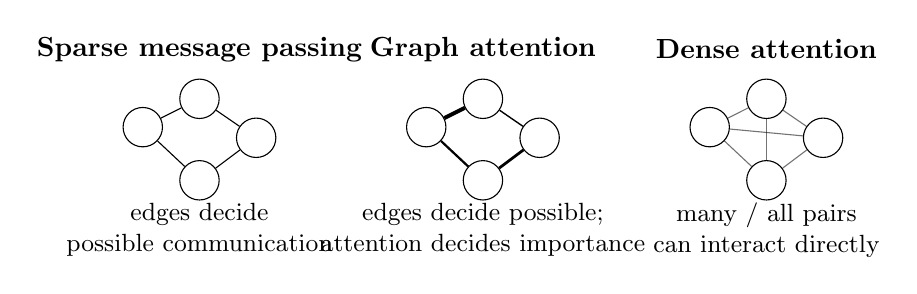
\begin{tikzpicture}[scale=0.9, every node/.style={font=\small}]
  \node[font=\bfseries] at (-4.0,2.0) {Sparse message passing};
  \node[font=\bfseries] at (0,2.0) {Graph attention};
  \node[font=\bfseries] at (4.0,2.0) {Dense attention};

  \foreach \offset in {-4,0,4} {
    \node[circle,draw,minimum size=5mm] (a\offset) at (\offset-0.8,0.9) {};
    \node[circle,draw,minimum size=5mm] (b\offset) at (\offset,1.3) {};
    \node[circle,draw,minimum size=5mm] (c\offset) at (\offset+0.8,0.75) {};
    \node[circle,draw,minimum size=5mm] (d\offset) at (\offset,0.15) {};
  }
  \draw (a-4)--(b-4)--(c-4)--(d-4)--(a-4);
  \draw[line width=1.4pt] (a0)--(b0);
  \draw[line width=0.5pt] (b0)--(c0);
  \draw[line width=1.0pt] (c0)--(d0);
  \draw[line width=0.8pt] (d0)--(a0);
  \draw[opacity=0.55] (a4)--(b4)--(c4)--(d4)--(a4);
  \draw[opacity=0.55] (a4)--(c4);
  \draw[opacity=0.55] (b4)--(d4);

  \node[align=center] at (-4,-0.55) {edges decide\\possible communication};
  \node[align=center] at (0,-0.55) {edges decide possible;\\attention decides importance};
  \node[align=center] at (4,-0.55) {many / all pairs\\can interact directly};
\end{tikzpicture}
\caption{Graph attention is a useful bridge between message passing and Transformer-style routing. Relaxing the sparse graph increases optional interaction paths but usually increases cost.}
\label{fig:gnn-to-transformer}
\end{figure}

\section{Failure mode: over-smoothing}
Neighbour mixing repeatedly pulls connected representations toward each other.
With enough smoothing-dominated layers, node states in a connected region can become difficult to distinguish, even if deeper receptive fields would in principle provide more context.
This is \textbf{over-smoothing}.

\[
\underbrace{\text{more message-passing depth}}_{\text{larger receptive field}}
\quad\Rightarrow\quad
\underbrace{\text{more repeated mixing}}_{\text{representations can converge}}
\quad\Rightarrow\quad
\underbrace{\text{less node-specific information}}_{\text{harder discrimination}}.
\]

Residual connections, normalisation, gating, decoupled propagation and shallower architectures can reduce the effect, but they do not make useful depth free.
Residual connections and normalisation are developed more generally in Section~8; here they act on a graph-specific problem created by repeated neighbourhood mixing.

\begin{figure}[htbp]
\centering
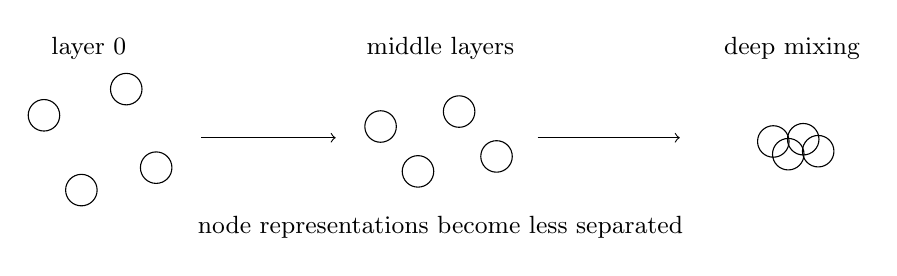
\begin{tikzpicture}[scale=0.95, every node/.style={font=\small}]
  \node at (-4.7,1.4) {layer 0};
  \node at (0,1.4) {middle layers};
  \node at (4.7,1.4) {deep mixing};

  \foreach \x/\y in {-5.3/0.5,-4.8/-0.5,-4.2/0.85,-3.8/-0.2} {
    \node[circle,draw,minimum size=4mm] at (\x,\y) {};
  }
  \foreach \x/\y in {-0.8/0.35,-0.3/-0.25,0.25/0.55,0.75/-0.05} {
    \node[circle,draw,minimum size=4mm] at (\x,\y) {};
  }
  \foreach \x/\y in {4.45/0.15,4.65/-0.02,4.85/0.18,5.05/0.02} {
    \node[circle,draw,minimum size=4mm] at (\x,\y) {};
  }
  \draw[->] (-3.2,0.2)--(-1.4,0.2);
  \draw[->] (1.3,0.2)--(3.2,0.2);
  \node at (0,-1.0) {node representations become less separated};
\end{tikzpicture}
\caption{Over-smoothing is representation collapse under repeated neighbourhood mixing. The diagram is conceptual: actual embedding geometry depends on the graph, parameters and training.}
\label{fig:gnn-oversmoothing}
\end{figure}

\section{Failure mode: over-squashing}
Over-squashing is different.
The problem is not that nearby node states become too similar; it is that information from a rapidly growing distant neighbourhood must be compressed through fixed-width states or narrow graph cuts before reaching the target.

\begin{figure}[htbp]
\centering
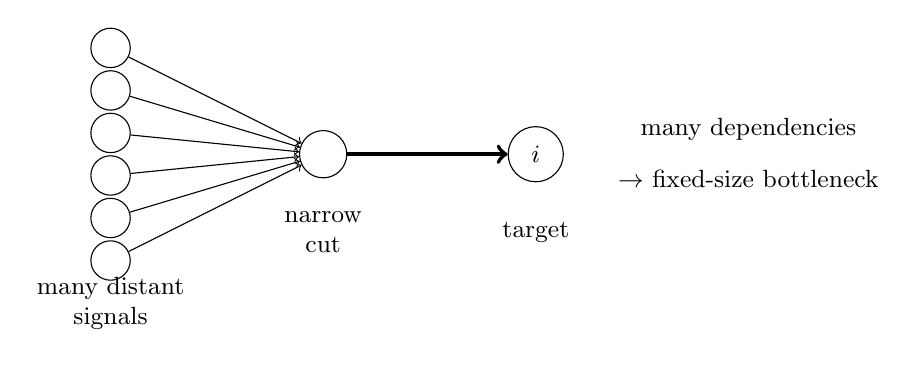
\begin{tikzpicture}[scale=0.9, every node/.style={font=\small}]
  \foreach \y/\k in {1.5/1,0.9/2,0.3/3,-0.3/4,-0.9/5,-1.5/6} {
    \node[circle,draw,minimum size=5mm] (l\k) at (-4.0,\y) {};
  }
  \node[circle,draw,minimum size=6mm] (b) at (-1.0,0) {};
  \node[circle,draw,minimum size=7mm] (t) at (2.0,0) {$i$};
  \foreach \k in {1,...,6} {\draw[->] (l\k)--(b);}
  \draw[->,line width=1.5pt] (b)--(t);
  \node[align=center] at (-4,-2.1) {many distant\\signals};
  \node[align=center] at (-1,-1.1) {narrow\\cut};
  \node[align=center] at (2,-1.1) {target};
  \node[align=left] at (5.0,0.35) {many dependencies};
  \node[align=left] at (5.0,-0.35) {$\rightarrow$ fixed-size bottleneck};
\end{tikzpicture}
\caption{Over-squashing: many distant dependencies are forced through a small information bottleneck. This can occur even when node representations have not over-smoothed.}
\label{fig:gnn-oversquashing}
\end{figure}

Increasing representation width, changing graph connectivity, adding long-range edges, using global attention or improving positional/structural information can help in different regimes.
These fixes target different mechanisms, so ``make the GNN deeper'' is often the wrong response to a long-range dependency problem.

\begin{calloutintuition}
Over-smoothing makes nodes too similar; over-squashing forces too much distant information through too little channel capacity.
\end{calloutintuition}

\section{Heterophily: neighbours need not look alike}
Many successful graph benchmarks are approximately \textbf{homophilic}: connected nodes often share labels or features.
Neighbour smoothing naturally fits that regime.
Other graphs are \textbf{heterophilic}: useful edges connect different roles, classes or states, such as buyers to sellers or reactants with complementary chemical roles.
In that case, blindly averaging neighbours can erase the distinction the task needs.

The architectural response may be relation-specific parameters, signed or directional messages, separate self and neighbour channels, higher-order structure, attention, or weaker reliance on direct neighbour similarity.
The correct question is therefore not whether graph connections exist, but what statistical meaning an edge has for the target.

\subsection{Inductive bias.}
If connected nodes should have related latent states, smoothing is useful; if edges encode complementarity rather than similarity, the message function must preserve that distinction instead of averaging it away.

\section{Graph construction can itself be learned}
A graph need not be fixed input data.
For point clouds, particles or latent representations, connectivity can be built from distance or similarity:

\[
\underbrace{\text{representations / coordinates}}_{\text{candidate entities}}
\rightarrow
\underbrace{\text{kNN / radius / learned affinity}}_{\text{construct edges}}
\rightarrow
\underbrace{\text{message passing}}_{\text{use edges}}.
\]

Recomputing neighbours after each representation update makes topology dynamic, allowing the interaction graph to evolve with the learned geometry.
This adds flexibility but couples representation learning to discrete or approximate neighbour selection, increasing instability and implementation cost.
A learned dense affinity moves still closer to self-attention: the boundary between ``GNN'' and ``Transformer'' becomes architectural rather than categorical.

\section{Geometry: invariance and equivariance}
Physical graphs often contain coordinates in addition to connectivity.
A molecular energy should not normally change because the molecule is translated or rotated; a predicted force vector should rotate with the molecule rather than remain numerically fixed.
This separates \textbf{invariance} from \textbf{equivariance}:

\[
\underbrace{f(Rx+t)}_{\text{transform input geometry}}
=
\begin{cases}
\underbrace{f(x)}_{\text{invariant scalar output}}, & \text{energy-like output},\\[2mm]
\underbrace{R f(x)}_{\text{equivariant vector output}}, & \text{force / direction-like output}.
\end{cases}
\]

Here $R$ is a rotation and $t$ a translation.
Equivariant GNNs constrain messages and features so these transformation rules hold by construction or by the chosen representation, rather than asking data augmentation alone to teach them approximately.
This is a strong inductive bias: it can improve data efficiency and physical consistency when the symmetry is correct, but it becomes a restriction when the environment contains a meaningful preferred orientation or reference frame.

\begin{figure}[htbp]
\centering
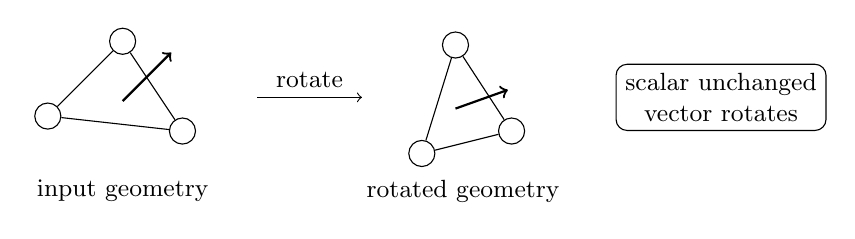
\begin{tikzpicture}[scale=0.95, every node/.style={font=\small}]
  \node[circle,draw] (a) at (-4,0) {};
  \node[circle,draw] (b) at (-3,1) {};
  \node[circle,draw] (c) at (-2.2,-0.2) {};
  \draw (a)--(b)--(c)--(a);
  \draw[->,thick] (-3,0.2)--(-2.35,0.85);
  \node at (-3,-1.0) {input geometry};

  \draw[->] (-1.2,0.25)--(0.2,0.25) node[midway,above] {rotate};

  \node[circle,draw] (d) at (1.0,-0.5) {};
  \node[circle,draw] (e) at (2.2,-0.2) {};
  \node[circle,draw] (f) at (1.45,0.95) {};
  \draw (d)--(e)--(f)--(d);
  \draw[->,thick] (1.45,0.1)--(2.15,0.35);
  \node at (1.55,-1.0) {rotated geometry};

  \node[draw,rounded corners,align=center] at (5.0,0.25) {scalar unchanged\\vector rotates};
\end{tikzpicture}
\caption{Geometric inductive bias can enforce the transformation behaviour the target should have rather than learning it separately for every orientation.}
\label{fig:gnn-equivariance}
\end{figure}

\section{Graph Transformers and structural encodings}
Dense self-attention does not automatically know which token pairs are adjacent in a graph.
Graph Transformers therefore inject structural information such as edge type, shortest-path distance, Laplacian coordinates, random-walk statistics or sparse attention masks.
These mechanisms answer a graph-specific version of the positional-encoding problem in Section~13.3: nodes form a set unless structure tells the model how one node is situated relative to another.

\begin{table}[htbp]
\centering
\small
\begin{tabular}{p{0.24\textwidth}p{0.34\textwidth}p{0.32\textwidth}}
\toprule
Structural signal & What it exposes & Main cost / caveat \\
\midrule
Graph edges / edge type & direct relations & misses long-range relation unless depth or global routing supplies it \\
Shortest-path distance & graph-relative separation & all-pairs preprocessing/storage can be expensive \\
Laplacian eigenvectors & global spectral coordinates & sign/basis ambiguities; graph-specific computation \\
Random-walk features & local-to-mesoscale connectivity statistics & additional preprocessing and scale choices \\
Global attention & direct long-range communication & can move complexity toward $O(N_{\text{nodes}}^2)$ interactions \\
\bottomrule
\end{tabular}
\caption{Graph Transformers trade stronger long-range access against additional structural machinery and, in dense forms, higher interaction cost.}
\label{tab:gnn-graph-transformer-structure}
\end{table}

A hybrid model can keep local message passing for cheap high-confidence relations and add a smaller amount of global attention for long-range dependencies.
This mirrors the broader sequence-model theme in Section~13.5: explicitly addressable interaction is expensive, while compressed or sparse communication is cheaper but more restrictive.

\section{Scaling: neighbourhood expansion and irregular memory access}
For a graph with average sampled branching factor $b$, naively expanding an $L$-layer neighbourhood around one target can touch roughly

\[
\underbrace{1+b+b^2+\cdots+b^L}_{\text{candidate nodes in an expanding computation graph}}
\]

nodes before duplicate overlaps are considered.
The problem is therefore not only arithmetic FLOPs; graph workloads also perform irregular gather/scatter operations over sparse neighbours, which can have poor memory locality compared with dense matrix operations.
Large-graph training commonly responds with neighbour sampling, subgraph/minibatch sampling, graph partitioning, cached embeddings or distributed storage.
Each method changes what information is available inside one optimisation step.

\begin{table}[htbp]
\centering
\small
\begin{tabular}{p{0.20\textwidth}p{0.34\textwidth}p{0.34\textwidth}}
\toprule
Scaling choice & Benefit & New cost \\
\midrule
Neighbour sampling & bounds fan-out per target & stochastic / incomplete neighbourhood \\
Subgraph sampling & batches locally connected regions & boundary information may be absent \\
Partitioning & distributes graph storage and compute & cross-partition communication \\
Sparse kernels & avoid dense $N_{\text{nodes}}^2$ work & irregular memory access and hardware dependence \\
Cached states & avoid repeated recomputation & staleness and invalidation-like consistency questions \\
\bottomrule
\end{tabular}
\caption{Large-graph systems trade complete neighbourhood information against tractable memory, communication and throughput.}
\label{tab:gnn-scaling}
\end{table}

\begin{calloutpracticaltip}
Profile sampled nodes/edges and memory traffic, not only parameter count; a small GNN can be bottlenecked by graph expansion and sparse data movement.
\end{calloutpracticaltip}

\section{Applications: the graph must encode a useful relation}
Graph structure is valuable when the relation itself carries predictive information.
The domain name is secondary to how entities, edges and targets are constructed.

\begin{table}[htbp]
\centering
\small
\begin{tabular}{p{0.18\textwidth}p{0.25\textwidth}p{0.25\textwidth}p{0.22\textwidth}}
\toprule
Domain & Nodes & Edges & Typical target \\
\midrule
Molecules & atoms & chemical bonds / geometric neighbours & molecular property, atom state, force \\
Recommendation & users/items or entities & interactions / relations & link likelihood, ranking feature, representation \\
Knowledge graph & typed entities & typed semantic relations & missing relation / entity prediction \\
Traffic network & road segments / sensors & physical connectivity & future traffic state \\
Meshes / PDEs & mesh cells / particles & adjacency / interaction radius & field update, dynamics, physical quantity \\
\bottomrule
\end{tabular}
\caption{A useful graph representation identifies entities and relations that align with the mechanism needed for prediction.}
\label{tab:gnn-applications}
\end{table}

For recommendation, graph methods complement rather than replace the two-tower and ranking systems in Sections~18--19: graph propagation can create richer user/item representations, while retrieval and ranking still solve the large-catalogue serving problem.
For scientific ML, graph meshes and particle systems connect directly to the physical inductive-bias discussion in Section~5.9.9.

\section{How GNN ideas evolved}
The useful history is a sequence of pressures on how graph information should move rather than a list of paper names.

\begin{table}[htbp]
\centering
\small
\begin{tabular}{p{0.15\textwidth}p{0.22\textwidth}p{0.25\textwidth}p{0.22\textwidth}}
\toprule
Stage & What changed & Pressure it addressed & New trade-off \\
\midrule
Spectral graph convolution & filters defined through graph-Laplacian structure & transfer convolution ideas to irregular domains & eigenbasis/global graph dependence can complicate scaling and transfer \\
Spatial message passing & update nodes from explicit neighbours & make locality and computation directly graph-local & long-range interaction requires depth \\
GCN-style simplification & normalised neighbourhood mixing + learned feature transform & simple scalable local baseline & smoothing bias can become restrictive \\
GraphSAGE / sampling & bounded sampled neighbourhoods & very large / evolving graphs & stochastic incomplete local evidence \\
GAT & learned neighbour weights & neighbours are not equally useful & extra attention cost \\
General MPNNs & richer node/edge messages & relations carry task-specific information & larger design and optimisation space \\
Geometric / equivariant GNNs & enforce physical transformation rules & coordinates and symmetries contain known structure & stronger assumptions, specialised operations \\
Graph Transformers / hybrids & add long-range attention + structural encodings & message-passing bottlenecks and global dependencies & denser interaction and structural-encoding cost \\
\bottomrule
\end{tabular}
\caption{A compressed evolution of GNNs: each stage changes the communication rule to address a limitation, while introducing a new cost or assumption.}
\label{tab:gnn-evolution}
\end{table}

The evolution is not a replacement chain.
GCNs remain useful baselines, sampling remains necessary at scale, equivariance matters only when the task has the relevant symmetry, and global attention is wasteful when local edges already capture the dependency structure.

\section{Research optionality: what exactly can be changed?}
A GNN experiment has design freedom at several distinct layers.
Keeping these layers separate prevents category errors such as treating neighbour sampling as an alternative to attention when the two can be used together.

\begin{table}[htbp]
\centering
\small
\begin{tabular}{p{0.26\textwidth}p{0.64\textwidth}}
\toprule
Design layer & Variables \\
\midrule
Graph construction & observed edges, kNN, radius, learned edges, direction, edge pruning, dynamic recomputation \\
Node / edge representation & raw features, embeddings, relation types, coordinates, temporal features, structural encodings \\
Message function & sender-only, sender+receiver, edge-conditioned, attention-weighted, geometric/equivariant \\
Aggregation & sum, mean, max, attention, degree normalisation, multi-aggregation \\
Update & MLP, residual, gated update, recurrent state, normalisation placement \\
Depth / range & message-passing layers, skip connections, long-range edges, global tokens/attention \\
Sampling / systems & fan-out, subgraph size, partitioning, sparse kernels, cache/staleness policy \\
Pooling / readout & sum/mean/max, set attention, hierarchical pooling, task-specific graph token \\
Objective & node, edge, graph loss; contrastive/self-supervised auxiliaries; negative sampling \\
Symmetry & permutation, translation/rotation invariance, equivariance group, coordinate frame \\
\bottomrule
\end{tabular}
\caption{The GNN research space is wider than choosing between named architectures. A paper usually changes one or a few rows of this table.}
\label{tab:gnn-optionality}
\end{table}

\subsection{Degree of experiment.}
Vary graph construction, neighbourhood radius/fan-out, representation width, message function, aggregation, attention, depth, residual/normalisation placement, edge features, structural encodings, pooling, symmetry constraints, sampling strategy and prediction objective.
Compare not only task quality but also sampled edges, memory traffic, latency/throughput and behaviour under graph perturbation or distribution shift.

\section{A diagnostic for choosing a GNN}
A graph architecture is attractive when the answer to several of the following questions is ``yes'':
\begin{enumerate}
  \item \textbf{Entities:} is the input naturally a variable-sized set of entities rather than a fixed grid or sequence?
  \item \textbf{Relations:} do known or constructible relationships identify likely information dependencies?
  \item \textbf{Reuse:} should the same local interaction rule apply across many nodes or edges?
  \item \textbf{Symmetry:} should arbitrary node ordering leave the function unchanged except for corresponding node-output reordering?
  \item \textbf{Range:} can useful evidence reach its target through a practical number of graph hops, or is global routing required?
  \item \textbf{Topology quality:} are the edges reliable enough to deserve architectural privilege?
  \item \textbf{Scale:} can the required neighbourhoods be sampled, partitioned or processed sparsely within the compute/memory budget?
\end{enumerate}

If relations are weak and arbitrary pairwise interaction is important, a set/Transformer architecture may be more natural.
If the data lie on a regular grid with strong translation-local structure, convolution may encode the same useful bias more cheaply.
If the target is mostly determined by independent node features, graph propagation can add cost and noise without buying useful information.

\begin{calloutintuition}
Use a GNN when edges are useful prior information about who should communicate; use attention more freely when the model must discover those routes from content.
\end{calloutintuition}

\section{Final mental model}
The reusable picture is one data flow:

\[
\boxed{
\begin{gathered}
\underbrace{\text{entities + relations}}_{\text{construct graph}}
\rightarrow
\underbrace{\text{messages along allowed routes}}_{\text{local communication}}
\rightarrow
\underbrace{\text{permutation-safe aggregation}}_{\text{compress neighbours}}
\\[1mm]
\downarrow
\\[-1mm]
\underbrace{\text{node / edge / graph readout}}_{\text{task output}}
\leftarrow
\underbrace{\text{updated node states}}_{\text{repeat for range}}
\end{gathered}
}
\]

The graph is therefore both data and inductive bias.
It can make sparse relational learning efficient by ruling out irrelevant interactions, but every ruled-out interaction is also a dependency the model must recover through longer paths, graph construction changes or a more global architecture.
